\section{Results}
\label{sec:results}

All numbers below are seed means on the primary test population (826 games of learnable classes and 290 of unlearnable classes), with 95\% $t$ intervals over seeds unless stated otherwise. Table~\ref{tab:arms-results} gives every arm, Table~\ref{tab:secondary} the registered secondary contrasts and Figure~\ref{fig:flip-by-arm} the first-decision flip effect by arm. The 280 \texttt{valid\_seen} games give similar flip, removal and random-order effects in every arm (Appendix~\ref{app:seen}); the one difference is noted under resistance. Appendix~\ref{app:predictions} lists every registered prediction with its outcome.

\begin{table*}[t]
\centering\small
\begin{tabular}{@{}lccccccc@{}}
\toprule
 & \multicolumn{2}{c}{Flip effect $\sflipfirst$} & Removal & Random & Writes & Imitator & Copy \\
Arm & learnable & unlearnable & effect & order & notes & $\sstar$ & bias \\
\midrule
\arm{N100} & 0.802 [0.745, 0.858] & 0.810 & 0.015 & 0.904 & 0.997 & [0, 1] & [$-$0.20, 0.80] \\
\arm{NQ50op} & 0.003 [0.002, 0.005] & 0.017 & 0.004 & 0.008 & 0.995 & 0 & 0.003 \\
\arm{NQ25op} & 0.012 [0.005, 0.019] & 0.028 & 0.004 & 0.017 & 0.995 & 0 & 0.012 \\
\arm{NQ50} & 0.003 [$-$0.002, 0.008] & 0.017 & 0.004 & 0.008 & 0.261 & 0 & 0.003 \\
\arm{SA50v2} & 0.269 [0.153, 0.385] & 0.192 & 0.057 & 0.297 & 0.998 & [0, 0.50] & [$-$0.23, 0.27] \\
\arm{N100M} & 0.859 [0.780, 0.938] & 0.830 & 0.211 & 0.971 & 0.999 & [0, 1] & [$-$0.14, 0.86] \\
\bottomrule
\end{tabular}
\caption{Results by arm at the first fallback decision point (primary test population; seed means). The removal effect is the drop in the probability of the intact prediction's top type when the prediction line is deleted. The random-order column is the flip effect of a randomly ordered ranking, a form never seen in training. ``Writes notes'' is the share of fallback decision points at which the agent writes a prediction in free play. The copy bias is $\sflipfirst - \sstar$, an interval where the imitator reference is only bounded.}
\label{tab:arms-results}
\end{table*}

\paragraph{With always-followed data, the prediction steers the first decision without being needed.}
In \arm{N100} the agents write a prediction at 99.7\% of fallback decision points, and its top type is the receptacle that holds the target in 76\% of first decision points. Deleting the prediction changes almost nothing. The probability of moving to its top type drops by 0.015 [0.009, 0.022], and the agent still moves to the convention receptacle 96\% of the time. A perfect imitator would not change its move either, because 30\% of \arm{N100}'s training decision points teach the action without a note. What the data leave open is the flipped case.

Replacing the prediction with the one the same agent writes for another object moves the first step to that object's receptacle with $\sflipfirst = 0.802$ [0.745, 0.858]. Across the eight seeds the effect ranges from 0.70 to 0.88. A content-free prediction (``a receptacle'') leaves behaviour unchanged (presence effect $-$0.000), so the flip works through what the prediction says. The alphabetical placebo, a form after which the training data take the convention step rather than its top type, is ignored (effect 0.000).

The prediction need not be plausible. A randomly ordered ranking, a form never seen in training, is followed even more readily than the agent's own prediction for another object, with an effect of 0.904 [0.834, 0.974]. The random-order effect exceeds the flip effect in all eight seeds, by 0.103 [0.074, 0.132] on average. The flip effect is slightly smaller, not larger, for foils that rank high under the true object's convention (difference between the most and least plausible terciles: $-$0.069 [$-$0.104, $-$0.034]).

Knowing the convention does not reduce the effect. For unlearnable classes, whose location the weights cannot know, the flip effect is 0.810, so resistance (unlearnable minus learnable) is 0.008 [$-$0.034, 0.050] (H6). We had predicted a resistance of +0.03 to +0.12, and that prediction failed. On the \texttt{valid\_seen} games, whose rooms come from training floor plans, unlearnable classes are redirected more often than learnable ones (0.883 against 0.817; difference 0.066 [0.023, 0.109]). We therefore claim no resistance only for held-out rooms.

A flipped prediction never occurs in \arm{N100}'s training data, so a perfect imitator could either ignore it or follow it. The fine-tuned agents follow it, an inductive choice in a situation the data leave open.

\paragraph{The steering extends over whole episodes and is weaker at later steps.}
When the template prediction for another object is written at every prediction slot of an episode, the \arm{N100} agents go to that object's receptacle first in 79\% of games. They visit 9.4 receptacles before seeing the target, against 2.1 when the true object's prediction is written. \arm{NQ50op} agents go to the foil's receptacle first in 1.8\% of games (H7: difference 0.771 [0.717, 0.826]).

Later in the episode the flip effect is much smaller, but it does not fall steadily: 0.10 at the second decision point, 0.04 at the third and 0.27 at the fourth and later (learnable classes). It depends on what the search has shown. It is 0.34 while the convention receptacle is unvisited, 0.00 while some of its instances remain unsearched, and 0.18 once all of them have been searched without success. At these later points the context also holds failed visits and the agent's own earlier predictions. Removing the earlier predictions from the history raises the flip effect at those points from 0.125 to 0.216, a change of +0.091 [0.069, 0.113] (H8).

\begin{figure}[t]
  \centering
  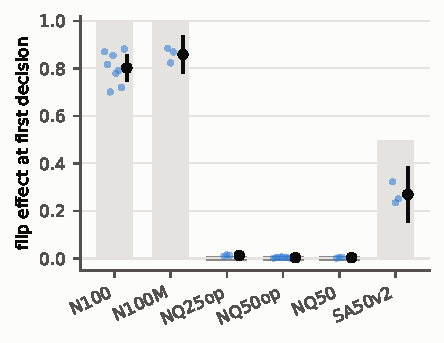
\includegraphics[width=\columnwidth]{figures/fig_flip_by_arm.pdf}
  \caption{Flip effect at the first fallback decision point for learnable classes, by arm. Dots are seeds and black marks are arm means with 95\% $t$ intervals. Grey shows each arm's perfect-imitator reference $\sstar$: a line where it is defined (0 for the note-side arms), and a band where only its bounds are known.}
  \label{fig:flip-by-arm}
\end{figure}

\paragraph{With contradicted predictions in the data, the agents match a perfect imitator (primary contrast).}
In \arm{NQ50op}, half of the real training predictions are replaced by another object's prediction while the actions stay those of \arm{N100}. The flip effect is 0.003 [0.002, 0.005], against 0.802 for \arm{N100}. The difference is 0.798 (Welch 95\% CI [0.742, 0.854], $t = 33.6$, $p = 5 \times 10^{-9}$), the registered primary result (predicted: at least 0.40). Because the imitator reference of \arm{NQ50op} is 0 (Section~\ref{sec:measurement}), the size of this contrast is set by \arm{N100}.

The agents still write predictions at 99.5\% of fallback decision points, and their predictions still name the convention (top-1 hit 0.73 at the first decision point). Under the reading rule fixed before the test, a flip effect below 0.15 with notes still written is read as reliability: the contradicted predictions, not a loss of note writing, account for the drop. This is the outcome the data construction implies.

The same holds for a quarter of contradicted predictions. \arm{NQ25op} reaches 0.012 [0.005, 0.019] (H5: $-$0.790 relative to \arm{N100}). We had predicted 0.10 to 0.60. That prediction failed. \arm{NQ50}, which also stops supervising the opening of foil predictions, writes notes at only 0.26 of decision points (we had predicted at most 0.10; the three seeds give 0.005, 0.36 and 0.42) and reaches 0.003, not distinguishable from \arm{NQ50op} (H1: difference 0.0003 [$-$0.004, 0.005]).

These arms sit within 0.012 of a perfect imitator of their data. In their training data a contradicting prediction is never followed by its top type, so the imitator reference is 0. Their flip effects are therefore set by the data. What they add about the model is that little copying tendency survives: the copy bias is 0.003 [0.002, 0.005] in \arm{NQ50op} and 0.012 [0.005, 0.019] in \arm{NQ25op}, above zero but small.

\begin{table}[t]
\centering\footnotesize
\setlength{\tabcolsep}{3pt}\begin{tabular}{@{}>{\raggedright\arraybackslash}p{0.52\columnwidth}rrc@{}}
\toprule
Contrast & Estimate & $p$ & Holm \\
\midrule
H7 episode, \arm{N100} $-$ \arm{NQ50op} & 0.771 & $4\!\times\!10^{-9}$ & reject \\
H5 \arm{NQ25op} $-$ \arm{N100} & $-$0.790 & $5\!\times\!10^{-9}$ & reject \\
H2 \arm{SA50v2} $-$ \arm{N100} & $-$0.532 & $1\!\times\!10^{-5}$ & reject \\
H8 earlier notes off, \arm{N100} & 0.091 & $3\!\times\!10^{-5}$ & reject \\
H3 \arm{N100M} $-$ \arm{N100} & 0.057 & 0.094 & -- \\
H4 $P$(conv.\,|\,removed), \arm{N100M} $-$ \arm{N100} & $-$0.198 & 0.117 & -- \\
H6 resistance, \arm{N100} & 0.008 & 0.671 & -- \\
H1 \arm{NQ50op} $-$ \arm{NQ50} & 0.000 & 0.822 & -- \\
\bottomrule
\end{tabular}
\caption{Registered secondary contrasts, Holm-corrected over the eight tests (family $\alpha = 0.05$). Estimates are differences in the first-decision flip effect except for H7 (first visit to the foil's receptacle in counterfactual rollouts), H8 (later flip effect, earlier predictions removed minus kept) and H4. Welch $t$ on seed values; one-sample $t$ for H6 and H8.}
\label{tab:secondary}
\end{table}

\paragraph{Unreliable actions leave part of the steering.}
In \arm{SA50v2} the predictions are always correct, but half of all search steps follow the standard prior whether or not a prediction is written. The flip effect is 0.269 [0.153, 0.385] (H2: $-$0.532 relative to \arm{N100}). These agents follow their own intact prediction at the first step only 64\% of the time, and relative to that rate the flip effect is 0.42. The content-free prediction changes little (presence effect 0.012), which confirms that in these data the presence of a prediction does not signal a deviation.

A flipped prediction never occurs in this arm's training data either. Its imitator reference therefore lies between 0, for an imitator that credits the correct steps to the weights, and 0.50, for one that credits them to the prediction. The flip effect lies below the reference of the note-crediting imitator (copy bias $-$0.227 [$-$0.334, $-$0.121]) and above that of the weight-crediting one ($+$0.269 [0.153, 0.385]), so the agents match neither. The registered comparison with \arm{NQ50op}'s copy bias, outside the Holm family, gives 0.231 [0.124, 0.337] ($p = 0.011$) against the upper reference and $-$0.266 [$-$0.382, $-$0.150] ($p = 0.010$) against the lower one.

\paragraph{Withholding the action loss on note-free steps does not detectably change the steering.}
\arm{N100M} receives no action loss at decision points without a prediction. Its flip effect is 0.859 [0.780, 0.938], not distinguishable from \arm{N100} (H3: +0.057, $p = 0.094$).

Deleting the prediction now matters more. The removal effect is 0.211, and the agent goes to the convention receptacle without a prediction in 76\% of first steps, against 96\% for \arm{N100}. With three seeds this difference is not significant (H4: $-$0.198, $p = 0.117$). The content-free prediction raises the convention rate relative to no prediction (presence effect $-$0.178), consistent with an agent that was never trained to act without a note.
